% !TEX root = ../thesis.tex
% [H] means put the figure HERE, directly when you input this code.
% Remove this to let LaTeX place the figure where it decides is best
\begin{figure}[H]
	\centering
	
% We use a figure width of 48.5% of the width of one line of text on 
% the page so there is some space between the images.
	\subfloat[Top-Left image sub-caption.]{
		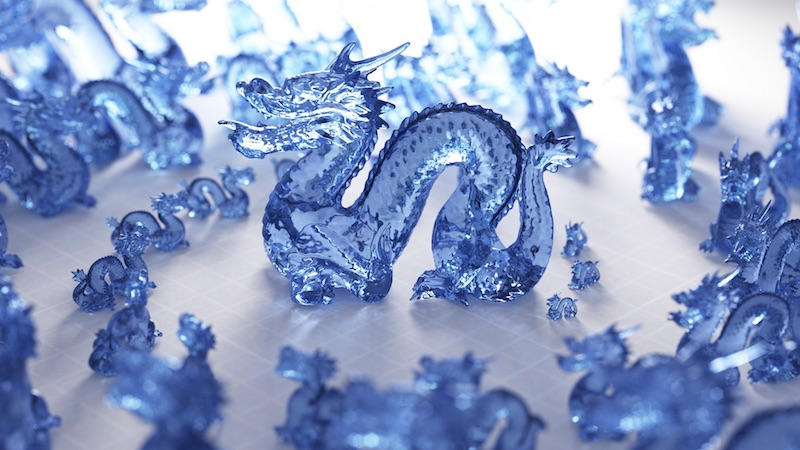
\includegraphics[width=0.485\textwidth]{dragon.jpg}\label{fig:example_2x2_a}
	}\hfill % Spacing between sub-figures displayed next to each other.
	\subfloat[Top-Right image sub-caption.]{
		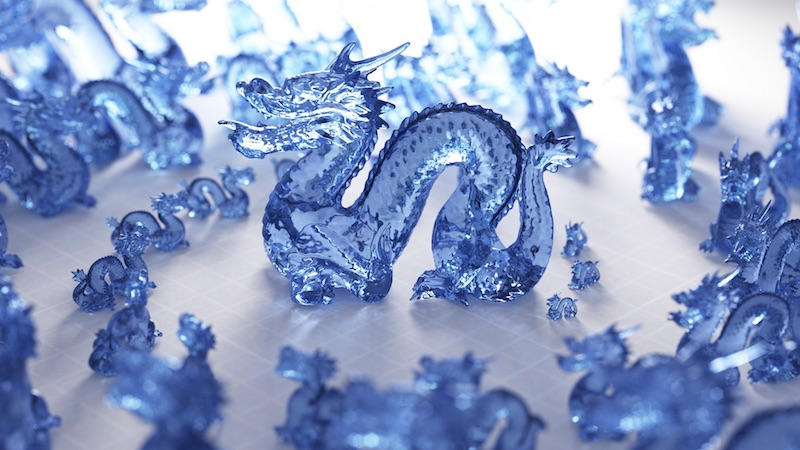
\includegraphics[width=0.485\textwidth]{dragon.jpg}\label{fig:example_2x2_b}
	}\\ % New line before caption.
	\subfloat[Bottom-Left image sub-caption.]{
		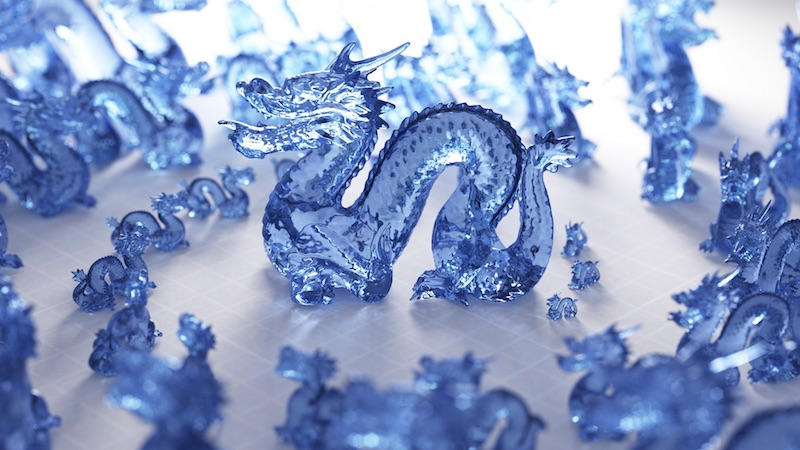
\includegraphics[width=0.485\textwidth]{dragon.jpg}\label{fig:example_2x2_c}
	}\hfill % Spacing between sub-figures displayed next to each other.
	\subfloat[Bottom-Right image sub-caption.]{
		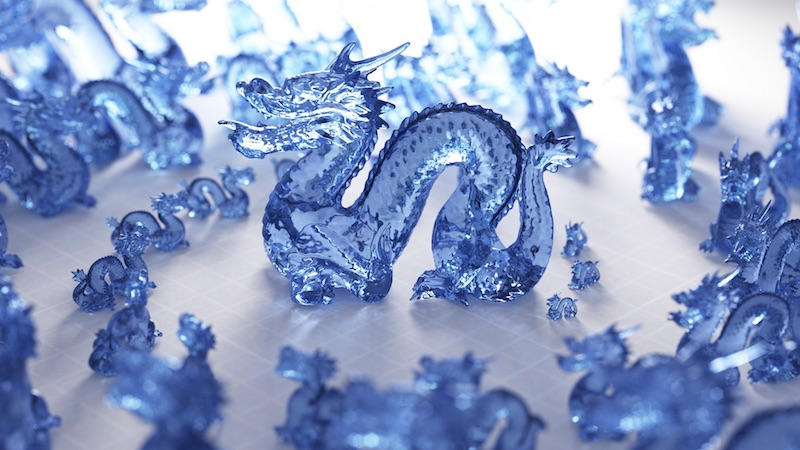
\includegraphics[width=0.485\textwidth]{dragon.jpg}\label{fig:example_2x2_d}
	}\\ % New line before caption.
		
% Caption is defined with a short and long version. The short version is shown in the 
% List of Figures section, and the long version is used directly with the figure. 	
	\caption[A demonstration of a 2x2 sub-figure layout.]{
A demonstration of a 2x2 sub-figure layout.
Between (a)--(b) and (c)--(d) we use \texttt{\(\backslash\)hfill} and between (b)--(c) we use a new line.
Image of glass dragons rendered using Path Tracing \cite{whittle15_dragons}.
	
% Figure labels should be defined at the end of the caption to ensure proper numbering.
	\label{fig:example_2x2}
	}
	
\end{figure}